\documentclass[runningheads]{llncs}

\usepackage[utf8]{vietnam}
\usepackage{graphicx}
\usepackage{hyperref}
\usepackage{amsmath,amssymb}
\usepackage{algorithm}
\usepackage{algpseudocode}
\usepackage{array}
\usepackage{multirow}
\usepackage{tabularx}

%\usepackage{biblatex}

% If you use the hyperref package, please uncomment the following line
% to display URLs in blue roman font according to Springer's eBook style:
% \renewcommand\UrlFont{\color{blue}\rmfamily}
%\addbibresource{jabref/references.bib}

\begin{document}
\newcolumntype{L}[1]{>{\raggedright\arraybackslash}p{#1}}
\newcolumntype{C}[1]{>{\centering\arraybackslash}p{#1}}
\newcolumntype{R}[1]{>{\raggedleft\arraybackslash}p{#1}}

\title{Tối ưu khoảng cách modified Hausdorff distance trong nhận dạng khuôn mặt người}
\titlerunning{Tối ưu khoảng cách MHD trong nhận dạng khuôn mặt}
%
%\titlerunning{Abbreviated paper title}
% If the paper title is too long for the running head, you can set
% an abbreviated paper title here
%
\author{Bùi Thanh Tính,
Trương Thiện Nhân}
%
\authorrunning{Bùi Thanh Tính, Trương Thiện Nhân}
\institute{}
% First names are abbreviated in the running head.
% If there are more than two authors, 'et al.' is used.
%
\institute{Khoa Điện-Điện tử, Trường Đại học Bách Khoa TP.Hồ Chí Minh\\
\email{\{buithanhtinh951,truongthiennhan3012\}@gmail.com}\\
Người hướng dẫn: ThS. Đặng Nguyên Châu}
%
\maketitle              % typeset the header of the contribution
%
\begin{abstract}
Khoảng cách Hausdorff là một công cụ được dùng để tính toán khoảng cách giữa hai tập hợp điểm. Phương pháp modified Hausdorff distance (MHD) đã ứng dụng khoảng cách Hausdorff để tính sự khác nhau giữa hai bản đồ cạnh của khuôn mặt và cho kết quả nhận dạng với kết quả tương đối tốt. Tuy nhiên, do độ phức tạp tính toán vốn có của nó, việc tính toán nguyên bản là rất khó khăn, không phù hợp với các hệ thống nhận dạng đòi hỏi tốc độ cao với cơ sở dữ liệu khổng lồ. Một thuật toán mới được chúng tôi đề xuất nhằm giảm khối lượng tính toán khoảng cách MHD. Chúng tôi đã vector hóa các điểm trội được trích ra từ ảnh, khoanh vùng dựa vào góc pha của chúng và tính toán trên các vùng đã được phân chia. Kết quả thí nghiệm chỉ ra rằng độ phức tính toán của phương pháp được đề xuất được cải thiện trong khi tỉ lệ nhận dạng ít thay đổi so với việc tính toán chính xác ban đầu.

\textbf{Từ khóa:} Nhận dạng khuôn mặt; khoảng cách Hausdorff; đặc trưng góc của các điểm trội; tối ưu khoảng cách MHD.
\end{abstract}
%
\section{Giới thiệu}
\label{Content: Gioi thieu}
~~~~Nhận dạng mẫu hình ảnh (pattern recognition) trong ảnh 2 chiều (2D) là một đề tài quan trọng trong lĩnh vực phân tích ảnh, nhận dạng vật thể và thị giác máy. Nhận dạng khuôn mặt được xem là một trong những phần quan trọng nhất của đề tài này và được rất nhiều nhà nghiên cứu quan tâm trong khoảng 20 năm qua. Nó có rất nhiều ứng dụng trong cuộc sống từ các ứng dụng chụp ảnh trên điện thoại, hệ thống bảo mật, cho đến những hệ thống an ninh cao cấp... Trong một hệ thống nhận dạng khuôn mặt, những đặc trưng của khuôn mặt được trích "offline" từ những ảnh gốc và được lưu trữ trong cơ sở dữ liệu các đặc trưng. Sau đó, trong bước nhận dạng, các đặc trưng mẫu được trích từ ảnh khuôn mặt ngõ vào, và so sánh với những đặc trưng của mỗi khuôn mặt trong cơ sở dữ liệu. Tuy nhiên, nếu số lượng ảnh gốc trong hệ thống là rất lớn thì việc tìm kiếm ảnh tương ứng trong cơ sở dữ liệu sẽ tốn nhiều thời gian. Những thuật toán tìm kiếm nhanh và hiệu quả là yêu cầu chung của các hệ thống nhận dạng.

Bản đồ cạnh khuôn mặt chứa những thông tin riêng biệt về hình dạng và cấu trúc khuôn mặt của những người khác nhau. Takács \cite{takacs1998comparing} là người đầu tiên đặt nền tảng cho việc sử dụng cạnh của khuôn mặt trong nhận dạng. Ông đã sử dụng khoảng cách modified Hausdorff distance (MHD) để so sánh sự giống nhau giữa các bản đồ cạnh, và chứng minh được rằng quá trình nhận dạng có thể bắt đầu sớm mà không cần các thuật toán trích đặc trưng cấp cao. Tuy nhiên, nhiều điểm trên cạnh có tính chất tương tự nhau và không có nhiều ý nghĩa cho việc nhận dạng. Sau khi dùng các phương pháp chọn lọc, các điểm trội trên cạnh đã được Y. Gao \cite{gao2003efficiently} sử dụng trong việc nhận dạng khuôn mặt. 

Việc sử dụng khoảng cách MHD trong nhận dạng khuôn mặt so sánh sự giống nhau tập hợp các điểm trội là một ứng dụng cụ thể của nó. Do đó, chúng tôi đã sử dụng những đặc điểm riêng biệt này để đưa ra một phương pháp tối ưu việc tính toán khoảng cách MHD trong quá trình nhận dạng. Nó đã làm giảm đáng kể khối lượng tính toán. Kết quả thử nghiệm cho thấy phương pháp đề xuất có độ phức tạp của thuật toán giảm khoảng 8 lần so với tính thuật toán tính MHD gốc và tỉ lệ nhận dạng thay đổi không đáng kể.

Phần còn lại của nội dung sẽ được trình bày như sau: Phần \ref{Content: Gioi thieu nhan dang khuon mat dung MHD} sẽ giới thiệu lại về khoảng cách MHD trong nhận dạng khuôn mặt sử dụng các điểm trội trên cạnh; phần \ref{Content: Phuong phap de xuat} sẽ trình bày về phương pháp đề xuất để tối ưu khoảng cách MHD trong nhận dạng khuôn mặt; Các mô phỏng và so sánh kết quả sẽ được trình bày trong phần \ref{Content: Thu nghiem va ket qua}; Nội dung bài báo sẽ kết thúc tại phần \ref{Content: Ket luan} với một số bình luận, đánh giá.

% -----------------------------------------------------------
%                        PHẦN 2
% -----------------------------------------------------------
\section{Nhận dạng khuôn mặt dựa vào bản đồ cạnh dùng MHD}
\label{Content: Gioi thieu nhan dang khuon mat dung MHD}

\subsection{Bản đồ cạnh khuôn mặt}
\label{ContentS: Ban do canh khuon mat}
~~~~Trong hệ thống nhận dạng khuôn mặt hiện nay, giai đoạn trích đặc trưng khuôn mặt là một trong những bước quan trọng nhất. Có rất nhiều cách để trích đặc trưng khuôn mặt, một trong những cách tối ưu nhất là bản đồ cạnh. Cạnh trong xử lý ảnh được định nghĩa là sự thay đổi giá trị mức xám đột ngột giữa các pixel. Cạnh là đặc trưng được trích dễ dàng bằng những phương pháp lọc cơ bản, nhưng lại rất hiệu quả trong nhận dạng, điều này rất phù hợp với các hệ thống yêu cầu tốc độ nhận dạng cao. Có nhiều phương pháp tìm cạnh trong một bức ảnh, mỗi phương pháp có những ưu nhược điểm khác nhau, tuy nhiên không có phương pháp nào là tối ưu hoàn toàn. Mỗi ảnh khác nhau có phương pháp tìm cạnh khác nhau. Chính vì thế, tùy vào từng trường hợp mà ta sử dụng các phương pháp tìm cạnh khác nhau. Những mô phỏng trong bài báo cáo này, chúng tôi sử dụng chương trình LEMGenerator của tác giả Y. Gao để tạo ra bản đồ cạnh cho một khuôn mặt. Trong chương trình này, tác giả sử dụng phương pháp tìm cạnh Babu, làm mỏng cạnh tạo các cạnh có độ dày một pixel và thuật toán Dynamic-two-Strip (Dyn2S) để tìm các điểm trội có nhiều tính chất đặc trưng nhất của cạnh. Kết quả một khuôn mặt sau khi qua chương trình sẽ được minh họa trong hình \ref{Fig: ban do canh}. Trong các mô phỏng ở phần \ref{Content: Thu nghiem va ket qua}, chúng tôi sử dụng các điểm này để tính toán.
\begin{figure}
\begin{center}
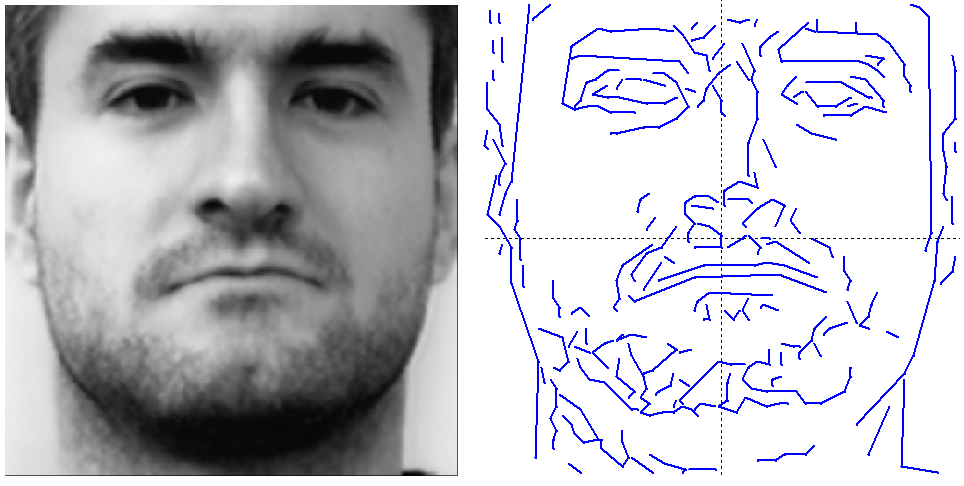
\includegraphics[scale=0.4]{figs/ban_do_canh.PNG}
\caption{Bản đồ cạnh của một khuôn mặt mẫu} \label{Fig: ban do canh}
\end{center}
\end{figure}


\subsection{Khoảng cách modified Hausdorff}
\label{ContentS: Khoang cach MHD}
~~~~Khoảng cách Hausdorff là một chỉ số (metric) so sánh hình dạng dựa trên ảnh nhị phân. Huttenlocher \textit{et al.} \cite{huttenlocher1993comparing} nhận định rằng khoảng cách Hausdorff cho so sánh ảnh nhị phân dễ chấp nhận nhiễu ở các vị trí của các điểm so với các kỹ thuật tương quan nhị phân khác, vì nó đo sự gần nhau hơn là tính chính xác. 

Cho A và B là hai tập hợp của các điểm trong không gian. Được đặt theo tên của Felix Hausdorff (1868-1942), khoảng cách Hausdorff $H(A,B)$  là khoảng cách lớn nhất trong hai khoảng cách Hausdorff trực tiếp $h(A,B)$ và $h(B,A)$ . Công thức toán học như sau:
\begin{equation}\label{Eq: HAB}
H(A,B)= max(h(A,B),h(B,A))
\end{equation}
với,
\begin{equation}\label{Eq: hAB}
h(A,B)=\max_{a \in A}(\min_{b \in B}(d(a,b)))
\end{equation}
Với $d(a,b)$  là khoảng cách euclid giữa hai điểm a,b. Hàm $h(A,B)$ được gọi là khoảng cách Hausdorff trực tiếp từ A đến B, là khoảng cách lớn nhất khi tính từ mỗi điểm $a \in A$  đến điểm  $b \in B$ gần nhất.

Dubuison và Jain \cite{dubuisson1994modified} đã đưa 24 dạng khác để tính toán khoảng cách Hausdorff và chỉ ra rằng MHD là khoảng cách tốt nhất. Khoảng cách MHD trực tiếp được định nghĩa như sau:
\begin{equation}
\label{Eq: hMHD_AB}
h_{MHD}(A,B)=\dfrac{1}{M}\sum_{a_{i} \in A}{\min_{b_{j} \in B}{d(a_{i},b_{j})}}
\end{equation}
Trong đó, M là số lượng điểm trong tập A. Định nghĩa không trực tiếp của MHD giống với công thức \ref{Eq: HAB}. Khoảng cách Hausdorff được định nghĩa bởi \ref{Eq: HAB} và \ref{Eq: hAB} rất nhạy cảm với các điểm nhiễu. Một vài điểm nhiễu, thậm chí chỉ một điểm cũng có thể làm thay đổi đáng kể giá trị khoảng cách, mặc dù 2 tập hợp điểm rất giống nhau. Khoảng cách MHD không chịu quá nhiều ảnh hưởng vì đặc tính giá trị trung bình trong công thức \ref{Eq: hMHD_AB} và số lượng không đáng kể của các điểm nhiễu. Thuật toán \ref{Alg: Khoang cach MHD truc tiep} trình bày phương pháp tính khoảng cách MHD trực tiếp.

\begin{algorithm}
\caption{Tính khoảng cách MHD trực tiếp}
\label{Alg: Khoang cach MHD truc tiep}
\begin{algorithmic}[1]
\Require Hai tập hợp hữu hạn điểm A và B với số lượng lần lượt là nA và nB.
\Ensure Khoảng cách MHD trực tiếp h(A,B).
    \State $sumA \gets$ 0
    \For{all ${a_i} \in$ A}
        \For{all ${b_j} \in$ B}
             \State $distA \gets dist(a_i, b_j)$ 
        \EndFor
        \State $sumA \gets sumA + min(distA)$ 
    \EndFor
    \State $hAB \gets sumA / nA$ 
    \State \textbf{return} $hAB$
\end{algorithmic}
\end{algorithm}

% -----------------------------------------------------------
%                        PHẦN 3
% -----------------------------------------------------------
\section{Phương pháp đề xuất}
\label{Content: Phuong phap de xuat}
\subsection{Đặc trưng góc của các điểm trội}
\label{ContentS: Dac trung goc}
~~~~Trước khi giới thiệu phương pháp, chúng tôi định nghĩa khái niệm đặc trưng góc của các điểm trội. Các điểm trội được trích từ ảnh khuôn mặt có những mối liên kết với nhau. Lợi dụng đặc điểm của tính chất này, chúng tôi thực hiện mã hóa với mỗi điểm trội được gắn vào một góc $\theta _i$ và phân loại những điểm này phụ thuộc vào $\theta _i$. Góc $\theta _i$ được tính như sau:

Cho tập hợp các điểm trội A gồm có \textit{m} điểm ${a_i}$ có tọa độ $(x_i,y_i)$, $i = \overline {1:m} $.
\begin{enumerate}
    % \item Gọi $d_{ik}^*$ là độ lớn khoảng cách từ điểm ${a_i}$ đến điểm ${a_k}$.

    % $$d_{ik}^* = \sqrt {{{({x_k} - {x_i})}^2} + {{({y_k} - {y_i})}^2}} $$
    \item Tính vector ${\vec v_{ik}}$ là vector từ điểm ${a_i}$ đến điểm ${a_k}$ và chuẩn hóa các vectors có độ lớn bằng 1.

    \[{\vec v_{ik}} = 1\angle {\tan ^{ - 1}}\frac{{{y_k} - {y_i}}}{{{x_k} - {x_i}}}\]
    \item Tính vector ${\vec v_i} = {V_i}\angle {\theta _i}$ đại diện cho điểm ${a_i}$.

    $${\vec v_i} = {V_i}\angle {\theta _i} = \sum\limits_{k = 1}^m {{{\vec v}_{ik}}} $$
\end{enumerate}

\subsection{Phương pháp được đề xuất}
\label{ContentS: Phuong phap duoc de xuat}
~~~~Khoảng cách MHD là một vấn đề về MAX - trung bình MIN. Điểm mấu chốt để giảm khối lượng tính toán chính là tính nhanh giá trị nhỏ nhất của từng điểm ở vòng lặp trong. Nghiên cứu của chúng tôi tập trung vào việc giảm số lần tính toán khoảng cách nhỏ nhất từ điểm $a_i$ thuộc tập hợp điểm A đến tất cả các điểm thuộc tập B. Khoảng cách MHD được tính toán để so sánh sự giống nhau giữa hai tập hợp điểm mà không cần sự tương ứng điểm - điểm như các khoảng cách khác, nghĩa là nó chỉ tìm điểm gần nhất về tọa độ thay cho điểm có tính chất tương đồng nhất. Do đó, chúng tôi lưu ý rằng để giảm khối lượng tính toán khoảng cách MHD cần phân loại trước những điểm trội thành nhiều nhóm, dựa trên những đặc trưng là mối liên hệ giữa các điểm trội với nhau, để giảm thiểu sự sai khác so với các tính thông thường. Trong bài báo này, chúng tôi sử dụng đặc trưng góc, đã được trình bày trong mục \ref{ContentS: Dac trung goc}.

Sau khi tính toán đặc trưng góc, chúng tôi thực hiện chia $360^o$ thành n khoảng có độ rộng góc bằng nhau. Dựa vào các đặc trưng góc đã tính toán, chúng tôi thực hiện sắp xếp câc điểm trội vào các khoảng đã chia. Khi tính toán khoảng cách từ điểm $a_i$ thuộc khoảng số \textit{class} của tập hợp điểm A đến tập hợp điểm B, chúng tôi chỉ tính khoảng cách từ $a_i$ đến các điểm có trong khoảng \textit{class} của tập B và lấy giá trị nhỏ nhất. Việc tính toán chỉ thực hiện một phần trong những điểm thuộc tập B nên khối lượng tính toán thuật toán của chúng tôi được cải thiện so với các tính trong thuật toán \ref{Alg: Khoang cach MHD truc tiep}. Thuật toán \ref{Alg: Khoang cach MHD truc tiep dung dac trung goc} trình bày các tính toán khoảng cách trực tiếp MHD.
\begin{algorithm}
\caption{Tính khoảng cách MHD trực tiếp dùng đặc trưng góc}
\label{Alg: Khoang cach MHD truc tiep dung dac trung goc}
\begin{algorithmic}[1]
\Require Hai mảng struct A, B gồm n phần tử, trong mỗi phần tử chứa tọa độ các điểm trội.
\Ensure Khoảng cách MHD trực tiếp h(A,B).
    \State $sumA \gets$ 0,\ $nA \gets 0$
    \For{$class=0;\ class < n;\ class++$}
    \For{all ${a_i} \in$ A(class)}
        \State $distA \gets 0$
        \State $nA \gets nA+1$
        \For{all ${b_j} \in$ B(class)}
             \State $distA \gets dist(a_i, b_j)$ 
        \EndFor
        \State $sumA \gets sumA + min(distA)$ 
    \EndFor
    \EndFor
    \State $hAB \gets sumA / nA$ 
    \State \textbf{return} $hAB$
\end{algorithmic}
\end{algorithm}

Giảm độ phức tạp của việc tính toán đồng nghĩa với việc chấp nhận sai số trong việc tính toán giá trị nhỏ nhất ở vòng lặp trong. Gao và Leung \cite{gao2002face} đã thêm vào công thức tính toán trong nghiên cứu của họ một thành phần gọi là chỉ số độ tin cậy. Áp dụng điều này vào tính toán khoảng cách MHD, chúng tôi thực hiện tính tổng số điểm $n_{A}$ nếu khoảng cách nhỏ nhất của điểm này ở vòng lặp trong nhỏ hơn K. Khi đó, độ tin cậy của bức ảnh được định nghĩa là:
\begin{equation}
\label{congthuc: R}
R=\dfrac{n_{A}}{n_{Atotal}}
\end{equation}
Thực hiện tương tự khi ta tính khoảng cách $h_{AB}$. Tổng tỷ lệ số điểm nằm ngoài vùng tin cậy của hai bức ảnh là:
\begin{equation}
\label{congthuc: Dn}
D_{n}=1-\dfrac{1}{2}\left(\dfrac{n_{A}}{n_{Atotal}}+\dfrac{n_{B}}{n_{Btotal}}\right)
\end{equation}
Vậy khoảng cách Hausdorff giữa hai bức ảnh sẽ là:
\begin{equation}
\label{Eq: H_MHDsuadoi}
H_{MHD}^*(A,B)=\sqrt{H_{MHD}^2(A,B)+(W_{n}D_{n})^2}
\end{equation}
Với $W_{n}$ là trọng số cho tổng số các điểm nằm ngoài vùng tin cậy.


\subsection{Độ phức tạp của tính toán}
\label{ContentS: Do phuc tap cua tinh toan}
~~~~Trong thuật toán \ref{Alg: Khoang cach MHD truc tiep}, có hai vòng lặp (vòng lặp trong và vòng lặp ngoài) và để đạt được kết quả thì phải thực hiện tính toán trên tất cả các điểm. Do đó, độ phức tạp của tính toán của thuật toán \ref{Alg: Khoang cach MHD truc tiep} là $O(nA*nB)$,với nA và nB lần lượt là số lượng điểm trong hai tập A, B.
Trong thuật toán \ref{Alg: Khoang cach MHD truc tiep dung dac trung goc}, nếu chia các đặc trưng góc thành n khoảng (n>1), độ phức tạp $O(nA*nB/2)$ xảy ra trong trường hợp xấu nhất khi tất cả các điểm nằm trên cùng một đường thẳng. Khía cạnh khác, trường hợp tốt nhất $O(nA)$ xảy ra khi $n \geqslant nB$, mỗi điểm trong tập B nằm trong những khoảng khác nhau. Trong trường hợp tổng quát, độ phức tạp tính toán được tính như sau:

Cho hai tập hợp điểm A, B có số điểm lần lượt là \textit{nA}, \textit{nB}, được chia thành n khoảng theo đặc trưng góc. Xác suất xuất hiện điểm trong các khoảng thứ \textit{i} của tập A là $q_{a_{i}}$, của tập B là $q_{b_{i}}$. Độ phức tạp khi tính khoảng cách từ A đến B là tổng độ phức tạp trên tất cả các khoảng $O(\sum_{i=1}^{n}{q_{a_{i}}*nA*q_{b_{i}}*nB})$.

% -----------------------------------------------------------
%                        PHẦN 4
% -----------------------------------------------------------
\section{Thử nghiệm và kết quả}
\label{Content: Thu nghiem va ket qua}
~~~~Trong phần này, chúng tôi thực hiện tính toán tỉ lệ chính xác việc nhận dạng với các điều kiện khác nhau của khuôn mặt: điều kiện lý tưởng, điều kiện ánh sáng và điều kiện góc chụp. Chúng tôi sẽ sử dụng khoảng cách MHD theo thuật toán \ref{Alg: Khoang cach MHD truc tiep} làm chuẩn để so sánh với thuật toán tính MHD theo đặc trưng góc đã đề xuất.

Chúng tôi sử dụng hai cơ sở dữ liệu chuẩn về khuôn mặt là Bern và AR để trích các điểm trội nhờ phần mềm LEMGenerator. Trong cơ sở dữ liệu Bern có ảnh của 30 người khác nhau, mỗi người sẽ có 10 ảnh xám (2 ảnh chụp chính diện, 2 ảnh đầu xoay sang trái, 2 ảnh đầu xoay sang phải, 2 ảnh ngước lên và 2 ảnh nhìn xuống). Trong cơ sở dữ liệu AR có ảnh của 100 người, gồm 50 nam và 50 nữ. Mỗi người sẽ có tất cả 26 ảnh khác nhau, trong đó có 13 ảnh gồm ảnh chụp trong điều kiện lý tưởng, điều kiện ánh sáng khác nhau, có mang các vật dụng và 13 ảnh còn lại giống điều kiện với 13 ảnh đầu nhưng được chụp sau 2 tuần. Tất cả các bức ảnh có kích thước 160x160.

Trong các mô phỏng, chúng tôi chia tập hợp các điểm trội thành 8 khoảng ($n=8$) và mô phỏng sự thay đổi của tỉ lệ nhận dạng khi Wn và K thay được. Kết quả như hình \ref{Fig: ti le nhan dang Wn K} được tính toán sử dụng các ảnh chính diện trong cơ sở dữ liệu AR. Từ hình \ref{Fig: ti le nhan dang Wn K}, chúng tôi lựa chọn $Wn=20$ và $K=4$ trong các mô phỏng.
\begin{figure}
\begin{center}
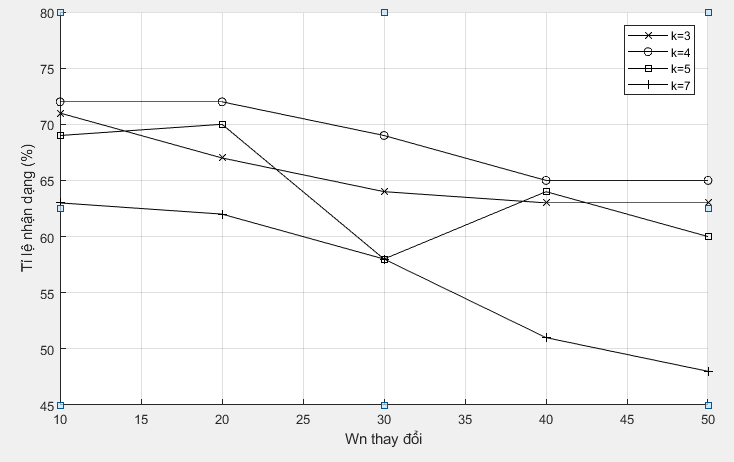
\includegraphics[scale=0.55]{figs/hinhWnK.PNG}
\caption{Tỉ lệ nhận dạng thay đổi theo Wn và K.} \label{Fig: ti le nhan dang Wn K}
\end{center}
\end{figure}


\subsection{Nhận dạng dưới điều kiện lý tưởng}
\label{ContentS: ketqualytuong}
~~~~Trong phần này, chúng tôi thực hiện tính độ chính xác của việc nhận dạng các hình ảnh, được chụp chính diện trong điều kiện lý tưởng thuộc hai cơ sở dữ liệu Bern và AR. Đối với cơ sở dữ liệu Bern, trong nhóm hình cùng một người, hình số 1 sẽ làm database và hình số 2 sẽ dùng cho việc nhận dạng. Đối với cơ sở dữ liệu AR, trong nhóm hình của cùng một người, chúng tôi chọn hình số 01 làm database và hình số 14 (được chụp trong điều kiện tương tự hình số 1 sau 2 tuần) làm hình cần nhận dạng. Kết quả thể hiện trong bảng \ref{Table: lytuong}.

\begin{table}[h]
\centering
\caption{Tỷ lệ chính xác việc nhận dạng với điều kiện lý tưởng.}
\label{Table: lytuong}
\begin{center}
\begin{tabular}{ |c||C{9em}|C{9em}|}
 \hline
 \multirow{2}{9em}{\centering{\textbf{Cơ sở dữ liệu}}} & \multicolumn{2}{c|}{\textbf{Phương pháp}} \\\cline{2-3} 
  & \textbf{MHD} & \textbf{MHD đề xuất}  \\\hline
 {} Bern & 100\% & 90\%     \\\hline
  AR   & 70\%  & 72\%        \\\hline
\end{tabular}
\end{center}
\end{table}
Đối với cơ sở dữ liêu Bern, tỷ lệ nhận dạng chính xác cao hơn nhiều so với tỷ lệ nhận dạng chính xác của cơ sở dữ liêu AR. Nguyên nhân dẫn đến điều này là do sự sai khác giữa ảnh cần nhận dạng và ảnh database, cơ sở dữ liệu Bern, hai ảnh được chụp cách nhau thời điểm rất ngắn sẽ ít sai khác, đối với cơ sở dữ liệu AR, hai ảnh được chụp cách nhau hai tuần và sẽ có nhiều thay đổi trên khuôn mặt.

\subsection{Nhận dạng trong điều kiện chiếu sáng khác nhau}
\label{ContentS: ketquachieusang}
~~~~Kết quả trong mục này, chúng tôi sử dụng cơ sở dữ liệu AR. Mỗi người sẽ được nhận diện trong 3 điều kiện ánh sáng bên phải (hình số 5 và hình số 18), ánh sáng bên trái (hình số 6 và hình số 19), ánh sáng cả hai bên (hình số 7 và hình số 20). Với mỗi điều kiện, một người sẽ có 2 bức ảnh, chúng tôi chỉ sử dụng một ảnh dùng cho nhận dạng và ảnh trong điều kiện lý tưởng làm database. Tổng cộng, chúng tôi sử dụng 600 ảnh để nhận dạng và 100 ảnh dùng làm database.

\begin{table}[h]
\centering
\caption{Tỷ lệ chính xác việc nhận dạng với điều kiện ánh sáng thay đổi.}
\label{Table: anhsang}
\begin{center}
\begin{tabular}{ |c||C{9em}|C{9em}|}
 \hline
 \multirow{2}{12em}{\centering{\textbf{Điều kiện chiếu sáng}}} & \multicolumn{2}{c|}{\textbf{Phương pháp}} \\\cline{2-3} 
  & \textbf{MHD} & \textbf{MHD đề xuất}  \\\hline
  Bên phải & 62\% & 62\%     \\\hline
  Bên trái   & 60\%  & 59.5\%        \\\hline
  Cả hai bên  & 47\%  & 40\%        \\\hline
\end{tabular}
\end{center}
\end{table}
Kết quả trong bảng \ref{Table: anhsang} cho thấy, trong điều kiện ánh sáng chiếu từ cả 2 bên, tỷ lệ nhận dạng chính xác giảm đáng kể. Khi đươc chiếu sáng nhiều, các đặc trưng cạnh bị mờ đi, sự thay đổi mức xám không nhiều ở các cạnh làm cho thuật toán trong chương trình LEM Generation không phát hiện được. Số điểm trội ít dẫn đến sai số lớn trong kết quả nhận dạng.

\subsection{Nhận dạng trong điều kiện góc chụp khác nhau}
\label{ContentS: ketquagocchup}
~~~~Mô phỏng trong mục này, chúng tôi chọn cơ sở dữ liệu Bern gồm có 30 người.  Mỗi người sẽ được nhận diện trong 4 trường hợp: nhìn sang trái (hình 3 và hình 4), nhìn sang phải (hình 5 và hình 6), nhìn lên trên (hình 7 và hình 8), nhìn xuống dưới (hình 9 và hình 10). Với mỗi điều kiện, một người sẽ có 2 bức ảnh cần nhận diện và dùng ảnh trong điều kiện lý tưởng làm database. Tổng cộng, chúng tôi sử dụng 240 ảnh để nhận dạng và 30 ảnh dùng làm database. Kết quả tỷ lệ chính xác được liệt kê trong bảng \ref{Table: gocchup}.

\begin{table}[h]
\centering
\caption{Tỷ lệ chính xác việc nhận dạng với điều kiện góc chụp thay đổi.}
\label{Table: gocchup}
\begin{center}
\begin{tabular}{ |c||C{9em}|C{9em}|}
 \hline
 \multirow{2}{10em}{\centering{\textbf{Hướng khuôn mặt}}} & \multicolumn{2}{c|}{\textbf{Phương pháp}} \\\cline{2-3} 
  & \textbf{MHD} & \textbf{MHD đề xuất}  \\\hline
  Nhìn sang trái & 53.33\% & 43.33\%     \\\hline
  Nhìn sang phải & 46.67\%  & 41.67\%        \\\hline
  Nhìn lên trên  & 60\%  & 40\%        \\\hline
  Nhìn xuống dưới  & 56.67\%  & 46.67\%        \\\hline
\end{tabular}
\end{center}
\end{table}
Thuật toán được đề xuất có kết quả nhận dạng thấp hơn nhiều so với thuật toán MHD bình thường. Nguyên nhân là thuật toán đề xuất phụ thuộc nhiều vào sự tương ứng về góc giữa các đặc trưng với nhau, do đó khi thay đổi góc chụp làm cho cấu trúc 3D của khuôn mặt biến dạng nhiều, và các cạnh trên khuôn mặt thay đổi đáng kể.

\subsection{Độ phức tạp của tính toán trên cơ sở dữ liệu cụ thể}
\label{ContentS: dophuctaptinhtoan}
~~~~Xác suất xuất hiện điểm trội trong các khoảng của khuôn mặt là không giống nhau, vì thế việc tính chính xác độ phức tạp của tính toán trong trường hợp tổng quát là không thể. Trong phần này, chúng tôi thực hiện tính toán cụ thể độ phức tạp của tính toán trên hai cơ sở dữ liệu BERN và AR. Chúng tôi lấy dữ liệu tương tự với phần \ref{ContentS: ketqualytuong}. 

\begin{table}[h]
\centering
\caption{Xác suất xuất hiện điểm trội.}
\label{Table: xacsuatxuathien}
\begin{center}
\begin{tabular}{ |c||C{3.5em}|C{3.5em}|C{3.5em}|C{3.5em}|C{3.5em}|C{3.5em}|C{3.5em}|C{3.5em}|}
 \hline
 \multirow{2}{6em}{\centering{\textbf{Bộ ảnh}}} & \multicolumn{8}{c|}{\textbf{Số thứ tự khoảng}} \\\cline{2-9} 
  & \textbf{1} & \textbf{2}  & \textbf{3} & \textbf{4} & \textbf{5} & \textbf{6} & \textbf{7} & \textbf{8} \\\hline
  BERN 1 & 0.1373 & 0.1255  & 0.1271   & 0.1343  & 0.0880   & 0.1551    & 0.1345   & 0.0983   \\\hline
  BERN 2 & 0.1379 & 0.1235  & 0.1273   & 0.1364  & 0.0875   & 0.1537    & 0.1384   & 0.0952   \\\hline
  AR 01  & 0.1706 & 0.1118  & 0.1024  & 0.1711  & 0.0811   & 0.1417    & 0.1415   & 0.0798   \\\hline
  AR 14  & 0.1706 & 0.1127  & 0.1012   & 0.1723  & 0.0802   & 0.1428   & 0.1432   & 0.0769   \\\hline
\end{tabular}
\end{center}
\end{table}
Trong bảng \ref{Table: xacsuatxuathien}, chúng tôi chọn ra những ảnh số 1 (BERN 1) và số 2 (BERN 2) của mỗi người trong cơ sở dữ liệu Bern, và chọn những ảnh số 01 (AR 01), 14 (AR 14) của mỗi người trong cơ sở dữ liệu AR (các ảnh chụp trong điều kiện lý tưởng). Sau đó, chúng tôi thực hiện tính tổng số các điểm trội trong mỗi khoảng đối với từng bộ ảnh, rồi lấy kết quả chia cho tổng số điểm trội trong bộ ảnh được xác suất xuất hiện các điểm trội trong từng khoảng thể hiện trong bảng \ref{Table: xacsuatxuathien}. Áp dụng kết quả độ phức tạp của tính toán trong mục \ref{ContentS: dophuctaptinhtoan} ta được kết quả: đối với cơ sở dữ liệu BERN, độ phức tạp của thuật toán đề xuất giảm đi 7.79 lần so với thuật toán ban đầu; đối với cơ sở dữ liệu AR, độ phức tạp của thuật toán đề xuất giảm đi 7.42 lần so với thuật toán ban đầu;
% -----------------------------------------------------------
%                        PHẦN 5
% -----------------------------------------------------------
\section{Kết luận}
\label{Content: Ket luan}
~~~~Cách tiếp cận nhận dạng khuôn mặt hiện nay yêu cầu các hệ thống máy tính thực hiện trên số lượng rất lớn các đặc trưng của khuôn mặt trong cơ sở dữ liệu và chọn ra những khuôn mặt phù hợp nhất. So sánh ảnh khuôn mặt sử dụng khoảng cách MHD là một trong những kỹ thuật nhận dạng nhanh. Một hệ thống có thể được xây dựng bằng cách xác định nhanh những khuôn mặt phù hợp, sau đó dùng các kỹ thuật có độ chính xác rất cao để để xác định khuôn mặt phù hợp nhất. Do đó, việc tính toán nhanh khoảng cách MHD là một vấn đề quan trọng và có thể không quá khắt khe với tỉ lệ chính xác.

Trong bài báo này, một phương pháp hiệu quả cho việc tính toán khoảng cách MHD được đề xuất. Trong phương pháp này, thay vì tính khoảng cách MHD trên tất cả các điểm thì các điểm trội được phân loại dựa trên đặc trưng về góc của chúng, và thực hiện tính toán trên những điểm được xem là tính chất góc gần giống nhau. Kết quả chỉ ra rằng phương pháp được đề xuất có khối lượng tính toán giảm 7.79 lần, tỉ lệ nhận dạng giảm 10\% đối với cơ sở dữ liệu BERN và giảm 7.42 lần, tỉ lệ nhận dạng tăng 2\% đối với cơ sở dữ liệu AR. Việc giảm khối lượng tính toán khoảng cách MHD bằng đặc trưng góc trong một phạm vi tỉ lệ nhận dạng thích hợp sẽ là bước đệm trong những phương pháp tính toán MHD nhanh dựa trên các đặc trưng khác trong tương lai, ứng dụng trong các hệ thống nhận dạng tốc độ cao.

\bibliographystyle{ieeetr}
\bibliography{jabref/references}{}
\end{document}